%%%%%%%% Applied Sciences (MDPI) --- Special Issue "Statistics in Data Science" %%%%%%%%
% Built as a free format submission, which Applied Sciences accepts: "We do not have strict
% formatting requirements, but all manuscripts must contain the required sections". Every required
% section is present and in the journal's order. MDPI's own template is deliberately not used:
% its licence says it "cannot be used for posting online on preprint servers or other websites",
% and this repository is public. Swap it in at revision, when the journal asks for the template.
%
% The ICML version of the same study is main.tex. The two share tables/, figures/ and main.bib.

\documentclass[10pt,a4paper]{article}

\usepackage[utf8]{inputenc}
\usepackage[T1]{fontenc}
\usepackage[a4paper,margin=2.5cm]{geometry}
\usepackage{lmodern}   % scalable: microtype's font expansion needs it, bitmap CM will not do
\usepackage{microtype}
\usepackage{graphicx}
\usepackage{subcaption}
\usepackage{booktabs}
\usepackage{amsmath}
\usepackage{amssymb}
\usepackage{mathtools}
\usepackage{amsthm}
\usepackage[numbers,sort&compress]{natbib}
\usepackage{hyperref}
\usepackage[capitalize,noabbrev]{cleveref}

\newtheorem{definition}{Definition}
\setlength{\parskip}{0.4em}
\renewcommand{\arraystretch}{1.1}

% The table files are shared with the ICML build, where two columns make table* the right
% environment. Here the document is one column, and a starred float is page-wide: LaTeX will only
% put it at the top of a page and defers it hard when it cannot, which is how the cohorts table
% ended up wedged between two references. Treat table* as an ordinary float, and let it sit where
% the text does by offering it every position rather than only the top.
\makeatletter
\renewenvironment{table*}[1][htbp]{\@float{table}[htbp]}{\end@float}
\makeatother

% The defaults reserve so much of a page for text that a large table is pushed forward rather than
% placed. These let a float take most of a page, which is what the wide tables here need.
\renewcommand{\topfraction}{0.9}
\renewcommand{\bottomfraction}{0.8}
\renewcommand{\textfraction}{0.07}
\renewcommand{\floatpagefraction}{0.75}
\setcounter{topnumber}{3}
\setcounter{bottomnumber}{2}
\setcounter{totalnumber}{4}

\title{\bfseries When Does Encoding Dynamics as Colour Help?\\
       Seven Handwriting Cohorts and an Acquisition Floor}

% [AUTHOR VERIFICATION REQUIRED]: confirm the authorship and the order of this study before
% sending. The list below is the VISAPP 2027 camera-ready's, carried forward.
\author{%
  Munif Gebara Jr.\,$^{1,*}$,\;
  \'Angel S\'anchez\,$^{2}$,\;
  Yandre Maldonado e Gomes da Costa\,$^{1}$,\\
  Igor Scaliante Wiese\,$^{3}$,\;
  Andr\'e Felipe Ribeiro Cordeiro\,$^{1}$,\;
  Jamily G.\ S.\ Souza\,$^{1}$\\[0.7em]
  \small $^{1}$\,Departamento de Inform\'atica, Universidade Estadual de Maring\'a,
    Maring\'a, PR, Brazil\\
  \small $^{2}$\,Departamento de Inform\'atica y Estad\'istica, Universidad Rey Juan Carlos,
    M\'ostoles, Madrid, Spain\\
  \small $^{3}$\,Departamento de Computa\c{c}\~ao, Universidade Tecnol\'ogica Federal do Paran\'a,
    Campo Mour\~ao, PR, Brazil\\[0.3em]
  \small $^{*}$\,Correspondence: munif@munif.com.br
}
\date{}

\begin{document}
\maketitle


\begin{abstract}
\noindent
A recurring recipe turns a sampled trajectory into an image for a vision model: the pen path is
drawn as ink, and a per-sample signal---speed, pressure, tilt---is painted along it as colour. It
is cheap and has been reported to work; when it works, and how much of a gain is the encoding, is
less clear. We apply one pipeline unchanged to seven handwriting cohorts, five clinical and two
non-clinical, with identical rendering, descriptors, nested cross-validation and statistics, and
every decision registered before any metric. The encoding gains
$+0.09$ to $+0.11$ macro F1 over the bare trace where the task fixes the figure and only execution
differs, and nothing where the produced shape carries the label. Giving each descriptor its
own baseline shows most of a reported margin is the descriptor, not the encoding: under a frozen
ImageNet backbone no cohort gains more than $+0.014$. A within-cohort test registered with its
direction beforehand was not confirmed, and is reported as a failure. Separately, a classifier
given two numbers containing no handwriting---the median sampling interval and the session clock
origin---reaches $0.97$ on one public clinical benchmark and $0.93$ on another. The quantity
carrying evidence is therefore the margin over this acquisition floor, not the score.
\end{abstract}

\noindent\textbf{Keywords:} handwriting; time series to image; benchmark validity; shortcut
learning; acquisition artefacts; nested cross-validation; preregistration; Parkinson's disease

\vspace{1em}

\section{Introduction}
\label{sec:intro}

\label{sec:intro}

Converting a time series to an image and classifying the image with a convolutional network is an
old idea with a steady stream of new instances. In the handwriting literature the specific form is
appealingly direct: the pen path is already two-dimensional, so it can be drawn as it was written,
and whatever else the digitiser recorded at each sample (speed, pressure, azimuth, altitude) can
be mapped onto the colour of the stroke at that point. The result preserves \emph{where} a dynamic
quantity occurred along the trace instead of aggregating it away, exactly what a vector of summary
statistics discards. We call such an image a \emph{pseudodynamic minimap},
following the formulation of \citet{prior2027minimaps}, whose single-cohort result this paper sets
out to transfer and test.

The appeal is obvious; the evidence is thinner than it looks. Published results are typically a
single cohort, a single acquisition device, and a comparison against a baseline chosen by the same
authors. That leaves two questions unanswered, and this paper is about both.

\paragraph{When does the encoding help?} An encoding that adds a channel cannot hurt in principle,
but it can in practice: it spends model capacity, it changes the texture statistics a descriptor
sees, and it can only pay for itself if the added channel carries information the shape does not.
We state that condition sharply and test it.

\paragraph{How would you know?} Clinical handwriting corpora are assembled over months, often with
patients and controls recruited through different routes and recorded in different sessions. Any
quantity that drifts with the session --- the sampling rate, the moment the clock started --- is
then correlated with the label without passing through the disease. \cref{sec:floor} measures how
far that goes.

\paragraph{Contributions.}
\begin{itemize}
\itemsep0em
\item \textbf{A transfer study with one pipeline.} Seven cohorts, identical rendering parameters,
descriptor, model grid, nested protocol and statistics; every design decision for every cohort
registered in a protocol document before any metric was computed
(\cref{sec:cohorts,sec:protocol}).

\item \textbf{A candidate rule, tested in both directions, and one failure reported as such.} The
minimap helps when the label is not in the shape, and not otherwise. Across cohorts this separates
the two gains from the three nulls; the one cohort built to hold both regimes falls between them on
the reported margin and with the nulls once each descriptor is given its own baseline.
\emph{Within} that cohort --- same children, tablet and session on both sides --- a
hypothesis registered with its direction before the splits were drawn is \textbf{not} confirmed:
the margin is larger on the half where the rule predicts none. We report the failure, and use the
floor below to bound what it can mean (\cref{sec:when}).

\item \textbf{Two mechanism controls, and a decomposition of the reported margin.} Shifting the
signal along each stroke and permuting it within each stroke destroy only \emph{where} the signal
sits; painting a channel that carries no information about the writer destroys only \emph{what} the
channel says. The first returns the gain to its baseline, the second does not reproduce it.
Separately, giving each descriptor its
own bare-trace baseline shows that the effect is the texture descriptor's alone: under a frozen
backbone no cohort gains more than $+0.014$, and most of the margin usually reported for this
recipe is the descriptor rather than the encoding (\cref{sec:results,sec:when}).

\item \textbf{The acquisition floor.} A two-feature classifier containing no handwriting reaches
$0.97$ inside one public clinical benchmark and $0.93$ on a second, where it beats every real arm;
on a third it matches four real pipelines including our own. We define the floor, give the
procedure, and report every result of the main table as a margin over it
(\cref{sec:floor,sec:results}).
\end{itemize}

We are explicit about what the floor result is not: not a claim that published models read the
clock, since our renderers never see an absolute timestamp, but a claim about what a number means.
A macro F1 of $0.93$ on a benchmark whose floor is $0.93$ is consistent with having measured nothing
about handwriting, and the reader currently has no way to tell.

\subsection{Related work}
\label{sec:related}

\label{sec:related}

\paragraph{Time series as images.} Encoding a sequence as a picture for an image model spans
recurrence plots \citep{eckmann1987recurrence}, Gramian angular fields and
Markov transition fields \citep{wang2015gaf}, and more recently direct rasterisations of
trajectories. The handwriting case differs in that the series already has a faithful
two-dimensional embedding, so the encoding does not have to invent a geometry: the question is only
what to do with the remaining channels.

\paragraph{Handwriting as a clinical signal.} Digitised handwriting has been used as a marker for
Parkinson's disease, for developmental dysgraphia and for cognitive decline
\citep{werner2006handwriting}. The dominant representation is a vector of kinematic and pressure
statistics \citep{drotar2016pahaw,drotar2020dysgraphia}; image-based alternatives are more recent,
and our baselines include both.

\paragraph{Shortcut learning and benchmark validity.} That models latch onto acquisition artefacts
rather than the phenomenon is well documented \citep{geirhos2020shortcut}, and in medical imaging
in particular, where scanner and site identity leak into diagnostic labels
\citep{degrave2021shortcut}. Our contribution is not the observation but the instrument: a floor
cheap enough to report with every result, and which we show is not a corner case in this domain.

\section{Materials and Methods}
\label{sec:methods}


\subsection{Pseudodynamic minimaps}
\label{sec:method}

\label{sec:method}

A recording is a sequence of samples $p_i = (x_i, y_i, t_i, c_i, \mathbf{s}_i)$, with position,
timestamp, a contact flag and a vector of per-sample signals. Only segments with contact at both
ends are drawn.

\paragraph{Geometry.} Contact points are fitted to a $512 \times 512$ canvas with a $20$~px margin,
preserving aspect ratio, and drawn as $4$~px line segments with $3\times$ supersampling followed by
Lanczos downsampling. A second geometry fixes the scale per task in device units instead of fitting
it per recording, so that absolute size is preserved across participants; its reference extent is
taken over every recording of that task without labels, which makes that arm transductive
(\cref{sec:geometry-appendix}). All cohort numbers reported here come from the canvas-fitted
geometry.

\paragraph{Colour.} For a chosen signal $s$ and segment $i$, the value is the mean of its endpoints,
$\bar{s}_i = (s_i + s_{i+1})/2$, normalised \emph{within the recording} by its own $5$th and $95$th
percentiles,
\begin{equation}
\tilde{s}_i = \mathrm{clip}\!\left(\frac{\bar{s}_i - q_{05}(s)}{q_{95}(s) - q_{05}(s)},\, 0,\, 1\right),
\end{equation}
and mapped affinely to a channel range $[30, 220]$. Speed is $\log(1+v)$ before normalisation;
azimuth is centred circularly before normalisation. Three signals can be assigned to the three
channels at once, giving the nine encodings we evaluate: the bare trace, four single-signal
minimaps (\textbf{S}peed, \textbf{P}ressure, \textbf{A}ltitude, a\textbf{Z}imuth) and four
triples (\cref{fig:examples}).

\begin{figure}[t]
\begin{center}
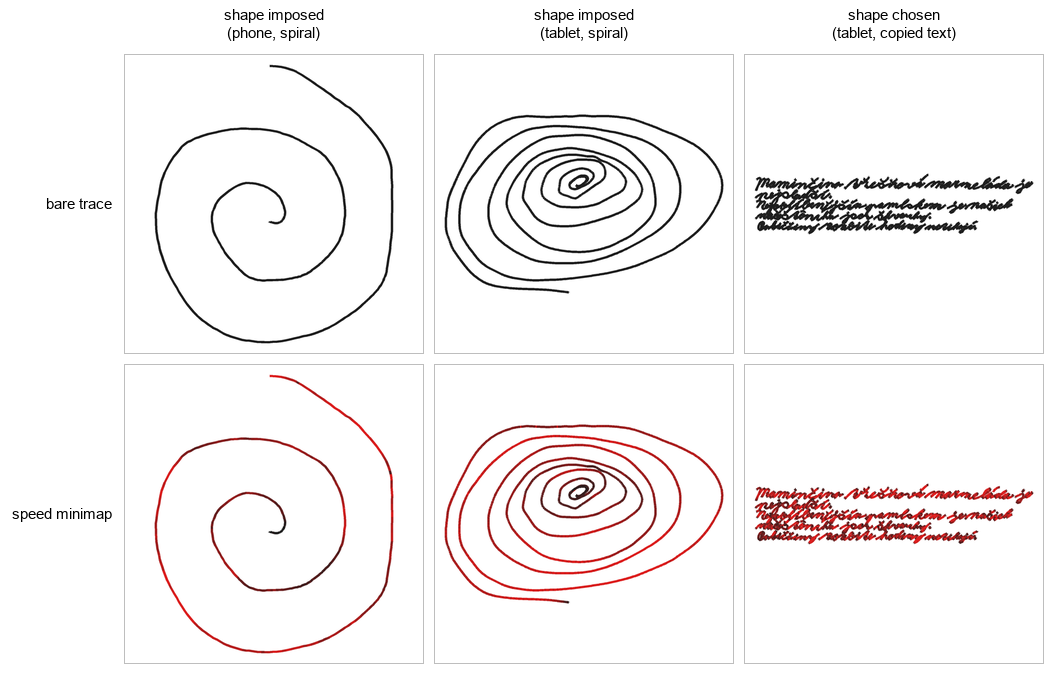
\includegraphics[width=\columnwidth]{figures/examples.png}
\end{center}
\caption{The same encoding on the two regimes of \cref{sec:when}, read from recordings the
experiments actually used. Left and centre: the task prescribes the figure, so the bare trace is
nearly the same for everyone and what differs is the execution the colour carries. Right: a copied
text, where the produced shape already carries most of what distinguishes one recording from
another, and where the square canvas shrinks a wide multi-line page into a strip. No participant is
identified and no panel was chosen for its appearance.}
\label{fig:examples}
\end{figure}

Two properties matter for the argument. The normalisation uses no statistic of the cohort and no
label, so nothing about the class distribution can enter the image; and the mapping is
\emph{positional}, the only part of the pipeline that records where along the trace a value
occurred, which is what \cref{sec:when} tests directly.

\paragraph{Descriptor and model.} Unless stated otherwise, images are described by Local Phase
Quantisation (LPQ) \citep{ojansivu2008lpq} on each channel ($64 \times 64$, $5\times 5$ window,
$256$ bins per channel, $768$ dimensions, square-root transformed) and classified by a support
vector machine. A frozen ImageNet ResNet18 \citep{he2016resnet} with an $\ell_2$-regularised
logistic head is the second descriptor over the identical images, which separates the encoding's
contribution from the descriptor's.

\subsection{Cohorts}
\label{sec:cohorts}

\label{sec:cohorts}

Seven cohorts, chosen to vary the instrument, the population and --- critically --- whether the
produced shape carries the label.

\paragraph{Shape fixed by the task.} In \textsc{ParkinsonHW} \citep{isenkul2013parkinsonhw} and
\textsc{Zhu} \citep{zhu2025smartphone} participants trace a
prescribed spiral or wave, so what differs between a patient and a control is execution, not
figure. \textsc{Zhu} is the extreme case of instrument change: a bare finger on a phone screen,
with no pressure and no angles, so the only minimap available is speed.

\paragraph{Shape chosen by the writer.} In \textsc{Drot\'ar--Dobe\v{s}}
\citep{drotar2020dysgraphia} and in the dictation and copy tasks of \textsc{DiaGraMo}
\citep{zvoncakova2026diagramo}, children write text; the produced shape varies with what was
written.

\paragraph{Both, under one setup.} \textsc{DiaGraMo} is the pivot of the study: the same children,
the same tablet and the same session produce ten graphomotor tasks whose target figure is imposed
and four whose shape is not, which lets the rule of \cref{sec:when} be tested without
changing anything else. It is the only cohort here that permits that test, and the one in which the
rule fails. Its own group has analysed this material with
direction-based fractional-order derivative features \citep{gavenciak2025fractional}; we cite that
work to place the cohort, and compare against the pipelines we ran ourselves rather than against
its reported numbers.

\paragraph{Non-clinical controls.} \textsc{SVC2004} \citep{yeung2004svc} is signature
verification: a skilled forger copies the shape deliberately, so only dynamics remain, the
cleanest positive control in this set. \textsc{Character Trajectories}
\citep{williams2006chartraj} is its mirror image: the label \emph{is} the shape, since a reader
identifies a character from ink alone.

\paragraph{Reference cohort.} \textsc{PaHaW} \citep{drotar2016pahaw} is the corpus on which the
encoding was originally reported \citep{prior2027minimaps}, and is included unchanged as a
regression control.

\subsection{Evaluation protocol}
\label{sec:protocol}

\label{sec:protocol}

Every cohort is evaluated identically, and every decision --- inclusion rule, task definition,
contact rule, unit conversion, split design --- was written into a per-cohort protocol document
\emph{before} any classifier was fitted on that cohort. Where the direction of the study changed
mid-stream, the protocol carries a dated addendum, not a rewrite.

\paragraph{Partitions.} Five repeats of five stratified outer folds, three inner folds for
selection, nested so that representation and hyperparameters are chosen on training participants
only. \textbf{The participant is the unit}: all recordings of a participant are in the same fold,
and participant decisions are the majority vote over the available tasks. Screening and
confirmation use disjoint master seeds; we treat split-to-split variation of $\pm 0.03$ macro F1 as
noise, and report no gain that does not reappear on the confirmation seed. That band was inherited
rather than measured; \cref{sec:splitnoise-appendix} measures it on twenty fresh seeds per cohort
and reports where it is too narrow.

\paragraph{Statistics.} Confidence intervals are $10{,}000$ label-stratified participant bootstrap
resamples. Paired contrasts use participant-wise swap randomisation. Multiplicity is corrected by
the Holm procedure \citep{holm1979} within families declared in the protocol.

\paragraph{Spatial controls.} To test whether a gain comes from \emph{where} the signal sits, we
apply two destructive controls at render time, each preserving every per-stroke marginal exactly:
a \emph{circular shift} of the signal values along each stroke, and a \emph{joint permutation} of
the signal values within each stroke. Both leave the ink and the colour histogram identical; only
the correspondence between position and value is destroyed.

\subsection{The acquisition floor}
\label{sec:floor}

\label{sec:floor}

\begin{definition}[Acquisition floor]
For a cohort $\mathcal{D}$ and an evaluation protocol $\Pi$, the acquisition floor
$\phi(\mathcal{D}, \Pi)$ is the score that $\Pi$ assigns to a classifier whose only inputs are
properties of the recording process that no behaviour of the subject can produce.
\end{definition}

We instantiate it with two features per recording: the \textbf{median sampling interval between
consecutive contact samples}, and $\log_{10}$ of the \textbf{first timestamp}, that is, the origin
of the session clock. Neither is a symptom: no disease makes a digitiser sample at $9$~ms instead
of $7$~ms, and none sets the clock. The second is independent of the writer by construction, the
first only approximately so, since a digitiser can drop samples under fast motion. That is one
reason to keep the probe to features whose dependence on behaviour is this weak, and to report wider
probes separately.

Either input can be a constant in a given release, and saying which is part of reading the floor:
the median interval varies in one of the six cohorts here and the clock origin in three, and
\cref{sec:cohorts-appendix} gives both columns. Where
both are constant the floor is at chance by construction, and the cohort is clean of these two
artefacts by inspection of two columns: a stronger statement than a classifier at chance, not a
weaker one. Where one varies the floor is effectively a one-feature probe: the $0.929$ reported
below on \textsc{Drot\'ar--Dobe\v{s}} is the session clock alone.

The floor is not chance: chance is a property of the label distribution, while the floor is a
property of the dataset as assembled and is the level below which a score is uninformative about the
phenomenon. We therefore report the margin $\Delta_\phi = \text{score} - \phi$ for every arm and
cohort, and treat it rather than the score as the quantity that carries evidence.

Measuring it costs nothing: it reuses the protocol already in place, and the features are two
reductions over a timestamp column. We report it for all six cohorts with a participant endpoint,
including those where our own results are positive.

\subsection{Use of generative AI}
\label{sec:genai}

Generative AI assistance was used in preparing this work and is disclosed here as the journal
requires. A large language model (Anthropic Claude) was used as a coding and editing assistant:
writing and reviewing analysis and rendering code, drafting and copy-editing the manuscript,
checking every bibliographic record against a registry, and auditing the reported numbers against
the run artefacts that produced them. It was not used to design the study, to choose hypotheses or
task subsets, to generate or impute data, or to interpret results; the protocol documents that fix
every design decision predate it and are dated. All code was executed by the authors, all outputs
were reviewed by the authors, and the authors take full responsibility for the content.
% Confirmed by the corresponding author on 2026-11-24 as matching how the tool was actually used
% across the project. Re-check before submission only if another tool is brought in, or if the
% division of labour changes during revision.


\section{Results}
\label{sec:results}

\label{sec:results}

\begin{table}[t]
\caption{Macro F1 at the unit level on the confirmation splits, which no model or encoding choice ever saw. $\Delta$ is the gain of the best minimap arm over the static trace; \emph{kinem.} is the 83 kinematic and pressure attributes computed from the same signals; \emph{floor} is the two-number acquisition classifier of \cref{sec:floor}, which contains no handwriting at all. $\Delta_\phi$, the margin over that floor, is the quantity that carries evidence: the score alone does not.}
\label{tab:headline}
\vskip 0.1in
\begin{center}
\begin{small}
\begin{tabular}{lrrrrrr}
\toprule
cohort & static & minimap & $\Delta$ & kinem. & floor & $\Delta_\phi$ \\
\midrule
ParkinsonHW$^{\dagger}$ & 0.757 & 0.925 & $+0.168$ & 0.854 & 0.666 & $+0.259$ \\
Zhu et al. & 0.627 & 0.879 & $+0.252$ & 0.843 & 0.473 & $+0.406$ \\
DiaGraMo & 0.658 & 0.708 & $+0.050$ & 0.716 & 0.453 & $+0.256$ \\
Drot\'ar--Dobe\v{s} & 0.767 & 0.777 & $+0.010$ & 0.783 & 0.929 & $-0.152$ \\
PaHaW & 0.634 & 0.636 & $+0.002$ & 0.650 & 0.642 & $-0.006$ \\
Char.\ Trajectories & 0.982 & 0.996 & $+0.015$ & 0.998 & 0.501 & $+0.495$ \\
\bottomrule
\end{tabular}
\end{small}
\end{center}
\vskip -0.1in
\end{table}


\cref{tab:headline} is to be read from the right. The score column says how a cohort behaves; the
$\Delta_\phi$ column says whether the behaviour is about handwriting.

\paragraph{Where the encoding gains, it gains under one descriptor.} On the two cohorts in which the
task dictates the figure, the best minimap arm beats the LPQ static trace by $+0.252$ on
\textsc{Zhu} and $+0.168$ on \textsc{ParkinsonHW}. Both sit far above their own floors
($\Delta_\phi = +0.406$ and $+0.259$), both exceed the $83$ kinematic and pressure attributes
from the identical signals, and both reproduce on the confirmation seed. Because
the two differ in almost everything --- a stylus on a graphics tablet against a bare finger on a
phone screen --- the behaviour is not a property of one digitiser.

%% Generated by scripts/x3_paper_tables.py from runs/. Do not edit by hand.
%% Every number below comes from the run that produced it. An edit here is silently overwritten
%% the next time the generator runs, and breaks the guarantee that no number in the paper can
%% differ from its run. To change a number, change the run or the generator.
\begin{table*}[t]
\caption{Each descriptor against its own bare trace, on the confirmation splits: the first three columns LPQ, the next three the frozen ResNet18, each $\Delta$ a minimap arm minus the static trace \emph{under the same descriptor and model grid}. \emph{descr.}\ is the remaining ingredient of the headline margin --- the identical bare trace, read by the backbone instead of by LPQ. Only the backbone's static arm is new; the other three reproduce \cref{tab:headline} exactly, on the same splits. Hypotheses, thresholds and the cohorts that can decompose into anything were registered before the run (addendum~F).}
\label{tab:within}
\vskip 0.1in
\begin{center}
\begin{small}
\begin{tabular}{lrrrrrrr}
\toprule
 & \multicolumn{3}{c}{LPQ} & \multicolumn{3}{c}{frozen ResNet18} & \\
\cmidrule(lr){2-4} \cmidrule(lr){5-7}
cohort & static & minimap & $\Delta$ & static & minimap & $\Delta$ & descr. \\
\midrule
ParkinsonHW$^{\dagger}$ & 0.757 & 0.843 & $+0.086$ & 0.911 & 0.925 & $+0.014$ & $+0.154$ \\
Zhu et al. & 0.627 & 0.736 & $+0.109$ & 0.893 & 0.879 & $-0.014$ & $+0.265$ \\
DiaGraMo & 0.658 & 0.637 & $-0.021$ & 0.720 & 0.708 & $-0.011$ & $+0.061$ \\
Drot\'ar--Dobe\v{s} & 0.767 & 0.777 & $+0.010$ & 0.825 & 0.762 & $-0.063$ & $+0.058$ \\
PaHaW & 0.634 & 0.636 & $+0.002$ & 0.619 & 0.630 & $+0.011$ & $-0.015$ \\
Char.\ Trajectories & 0.982 & 0.989 & $+0.008$ & 0.995 & 0.996 & $+0.001$ & $+0.013$ \\
\bottomrule
\end{tabular}
\end{small}
\end{center}
\vskip -0.1in
\end{table*}


Those two numbers are not the size of the encoding effect, and \cref{tab:within} says why. Both
compare the best minimap arm, which on these cohorts is the frozen backbone, against a static trace
described by LPQ: the comparison changes the painted channel \emph{and} the descriptor at once.
Against the bare trace under its own descriptor the encoding is worth $+0.086$ and $+0.109$ under
LPQ (which is also where the controls of \cref{sec:when} locate it) and $+0.014$ and $-0.014$
under the backbone. Of those two LPQ margins only \textsc{Zhu}'s separates from zero (CI $+0.036$ to
$+0.189$, Holm $p = 0.018$); on \textsc{ParkinsonHW}, with $51$ participants, the interval is
$-0.002$ to $+0.176$ (Holm $p = 0.26$). The rest is the descriptor, and it separates from zero on
both. We keep $\Delta$ in \cref{tab:headline} because it is the quantity every experiment here
compared, and print $\Delta_w$ beside it because it is the quantity about the encoding; the arms,
the thresholds and the direction of this test were registered before it ran.

\paragraph{The descriptor advantage is not a constant.} If a pretrained backbone simply read bare
traces better than LPQ, the \emph{descr.}\ column of \cref{tab:within} would be flat. It is not: it
runs from $-0.015$ on \textsc{PaHaW}, the cohort the encoding was first reported on, to $+0.154$ and
$+0.265$ on the two that carry the headline gains. The backbone's advantage on a bare trace is
largest exactly where $\Delta$ is largest, which is
the uncomfortable reading of the table: what those two cohorts have and the others do not is a
static trace that suits ImageNet features, and most of $\Delta$ measures that, not the painted
channel.

\paragraph{Where the shape carries the label, the encoding does nothing.} The margins are
$+0.010$ on \textsc{Drot\'ar--Dobe\v{s}}, $+0.002$ on \textsc{PaHaW} and $+0.015$ on
\textsc{Character Trajectories} ($+0.008$ under LPQ, $+0.001$ under the backbone), all inside the
$\pm 0.03$ band we declared as split noise. Of the three, only
\textsc{Drot\'ar--Dobe\v{s}} depends on the split: twenty fresh master seeds put its margin at
$+0.032$ on average, every one of them above the $+0.010$ we drew, so that cohort is the band's
edge rather than its middle (\cref{sec:splitnoise-appendix}). Only the character null was
registered in advance as a directional hypothesis; the other two were not. The character cohort is
the sharpest because every arm is above $0.98$: a reader identifies a character from ink alone, so
there is nothing for dynamics to add. Restoring headroom there --- the canonical $20$-class problem
instead of the three declared pairs, registered as Addendum~A before it ran
(\cref{sec:cohorts-appendix}) --- leaves $+0.012$, an order of magnitude below the Parkinson
cohorts. A real effect, and a negligible one.

\paragraph{Absolute size matters, but no reported number depends on it.} The screening step
renders every available encoding under both geometries, and the paired contrast between them spans
$-0.080$ to $+0.108$ macro F1 at the participant endpoint over $37$ comparisons, $15$ of them past
the $0.03$ rule, with the direction belonging to the cohort rather than to the geometry
(\cref{sec:geometry-appendix}). Choosing a geometry per cohort on that evidence is the hindsight
this protocol refuses, so the geometry joins the encoding as a training-only choice, picked by the
inner loop in two further arms at the confirmation seed. There the fixed scale moves the selected
arms by $-0.034$ to $+0.021$ across the
four cohorts that carry them, a single move outside the band. We therefore render at the
canvas-fitted geometry throughout. No reported number depends on that choice, which is a narrower
claim than absolute size carrying nothing.

\paragraph{The positive control behaves as the rule predicts.} \textsc{SVC2004} is the limiting
case: a skilled forger copies the shape on purpose, so the shape is uninformative by construction.
The static trace is at chance ($0.491$ macro F1) and all eight encodings carrying a signal score
above it, up to $0.653$ (\cref{sec:signature-appendix}). It has neither a participant endpoint nor a
floor (a forger and a genuine signer are not two groups of people), so it is evidence about the
rule, not about clinical performance.

\paragraph{On two cohorts the floor swallows the result.} On \textsc{Drot\'ar--Dobe\v{s}} two
numbers that contain no handwriting score $0.929$ against the minimap's $0.777$ and the kinematic
attributes' $0.783$: $\Delta_\phi = -0.152$, and every pipeline we ran there is worse than its
clock. On \textsc{PaHaW} the floor is $0.642$ against $0.636$, $0.630$, $0.650$ and $0.634$ for the
two minimaps, the kinematic attributes and the bare trace: four pipelines and an artefact,
indistinguishable.
\textsc{ParkinsonHW} is the case that forced us to define the floor at all. Inside its
\texttt{hw\_dataset} release the two features reach $0.973$, because the digitiser's sampling period
separates those patients from everything else; the sub-cohort that remains once they are removed
($36$ patients and $15$ controls) is the one reported here, and on it the minimap keeps $+0.259$
over the floor. The artefact therefore does not explain that cohort's gain, but without measuring
it we could not have known, and a result on the whole release would be computed partly on recordings
that two numbers separate at $0.973$.

\paragraph{A narrow floor is not a clean cohort.} Widening the deliberately minimal probe to six
acquisition descriptors --- adding sample count, duration and two contact-interval statistics, none
of them a property of the writing --- changes the picture twice: it reaches $0.784$ on
\textsc{DiaGraMo}, above every image arm and above the kinematic attributes ($0.716$), and $1.000$
on \textsc{Character Trajectories}, whose two narrow features are both constant and whose floor is
therefore at chance. Duration and sample count encode how long a character takes to write, which
legitimately identifies it, so we keep the floor narrow enough that no behaviour of the writer can
move it and report the six-feature arm as an upper bound, not a floor.

\subsection{When the encoding helps}
\label{sec:when}

\label{sec:when}

\paragraph{The rule.} The pattern in \cref{tab:headline} separates the cohorts into two groups: the
minimap gains where the produced figure is imposed by the task and the label lives in the execution
($+0.168$ and $+0.252$, or $+0.086$ and $+0.109$ within the descriptor that carries them), and gains
nothing where the produced shape itself carries the label ($+0.010$, $+0.002$ and $+0.015$, or
$+0.010$, $+0.002$ and $+0.008$ under LPQ, the column of \cref{tab:within} in which an encoding gain
exists at all). The ordering is the same under either column, which is why the rule is stated from
the pattern rather than from the size of any one gain. It also survives redrawing the splits a
hundred times, the two groups never once overlapping (\cref{sec:splitnoise-appendix}).
\textsc{PaHaW} sits in the second group because seven of its eight
tasks are writing, although the first is a spiral; its null is also level with its floor, so it
weighs little either way. \textsc{DiaGraMo}, whose fourteen task slots mix the two regimes, falls
between the groups at $+0.050$, where a mixture should fall. But its within-descriptor margin
under LPQ is $-0.021$, which puts it with the nulls instead, and fresh splits agree
(\cref{sec:splitnoise-appendix}). Its intermediate position is therefore an artefact of the
baseline, and the cohort built to interpolate between the two regimes does not. The signature cohort
extends the rule to a non-clinical label and the character cohort anchors its null end: a regularity
over seven datasets, stronger than the single-cohort evidence this recipe is usually reported with
and weaker than a controlled test, since acquisition, population and task change together between
cohorts.

\begin{table}[t]
\caption{Spatial controls on the LPQ selection arm, screening splits. Both destroy only the correspondence between position along the stroke and signal value, leaving the ink, the contact mask and every per-stroke marginal identical. A cost means the classifier reads \emph{where} the signal sits along the trace; no cost means it reads only how the values are distributed.}
\label{tab:controls}
\vskip 0.1in
\begin{center}
\begin{small}
\begin{tabular}{lrrrrr}
\toprule
cohort & minimap & shift & permuted & $\delta$ shift & $\delta$ perm. \\
\midrule
ParkinsonHW$^{\dagger}$ & 0.738 & 0.637 & 0.624 & $-0.101$ & $-0.114$ \\
Zhu et al. & 0.750 & 0.688 & 0.649 & $-0.062$ & $-0.101$ \\
DiaGraMo & 0.645 & 0.669 & 0.648 & $+0.024$ & $+0.003$ \\
Drot\'ar--Dobe\v{s} & 0.783 & 0.758 & 0.772 & $-0.025$ & $-0.011$ \\
PaHaW & 0.590 & 0.586 & 0.607 & $-0.004$ & $+0.017$ \\
Char.\ Trajectories & 0.989 & 0.985 & 0.989 & $-0.004$ & $+0.000$ \\
\bottomrule
\end{tabular}
\end{small}
\end{center}
\vskip -0.1in
\end{table}


\paragraph{The gain is positional.} \cref{tab:controls} removes the one thing the encoding adds:
both controls keep the ink, the contact mask and every per-stroke colour marginal identical, and
destroy only the correspondence between position along the stroke and signal value. Every column is
from the same run, so each row reads against its own static baseline. Where there is a gain, both
controls return the score to that baseline, on \textsc{ParkinsonHW} from a $+0.098$ margin and on
\textsc{Zhu} from $+0.067$; where there is none there is nothing to remove, and the controls move
the score by less than the noise band in either direction: on \textsc{DiaGraMo} the shift is
nominally \emph{better} than the authentic images. So the LPQ gain,
where it exists, comes from \emph{where} along the trace a value occurred and not from the
distribution of values, which is the only thing a minimap encodes that a summary vector does not.
The larger ResNet18 gains of \cref{tab:headline} have been put through the same controls on
\textsc{DiaGraMo}, reported below; on the two cohorts that carry the cross-cohort gain they have
not.

\paragraph{A channel that contains nothing.} Both controls above still paint the real signal, so
neither can tell whether a gain comes from what the channel contains or from the act of adding a
channel that varies at all. We therefore
paint channels that carry no information about the writer and change nothing else: a ramp, an AR(1)
sequence matched to that recording's own smoothness, and white noise, all three rendered through the
identical normalisation (\cref{sec:controls-appendix}). The direction was registered before the run,
with the threshold at which we would have concluded that the encoding's benefit is the channel
addition rather than its content.

On \textsc{Zhu}, which carries the largest reported gain and has one dynamic signal so that no
selection enters the comparison, the control passes under LPQ: the real speed channel gains $+0.109$
over the static trace (CI $+0.036$ to $+0.189$) while the three nulls gain $+0.029$, $-0.015$ and
$-0.012$, every interval across zero. Under the frozen backbone the question has no content, that
descriptor having no encoding gain here to explain. What a minimap paints matters to the local
descriptor and not to the backbone.

\begin{table*}[t]
\caption{The contrast inside DiaGraMo: the same children, the same tablet, the same session. Ten tasks impose the target figure, four do not, and the direction was registered before the splits were drawn. It came out backwards, and the \emph{nuisance} column --- six acquisition descriptors, no handwriting in them --- shows why that outcome cannot be read as evidence about pen dynamics.}
\label{tab:diagramo}
\vskip 0.1in
\begin{center}
\begin{small}
\begin{tabular}{lrrrrrr}
\toprule
task set & static & LPQ & ResNet18 & $\Delta$ best & floor & nuisance \\
\midrule
all 14 tasks & 0.658 & 0.637 & 0.708 & $+0.050$ & 0.453 & 0.784 \\
graphomotor (10) & 0.616 & 0.599 & 0.647 & $+0.030$ & 0.432 & 0.593 \\
writing (4) & 0.635 & 0.623 & 0.703 & $+0.069$ & 0.424 & 0.846 \\
\bottomrule
\end{tabular}
\end{small}
\end{center}
\vskip -0.1in
\end{table*}


\paragraph{The within-cohort test, and its failure.} The cross-cohort rule invites one controlled
experiment, and \textsc{DiaGraMo} supplies it: $273$ children and $3{,}796$ recordings on one
tablet in one session, ten task slots imposing the target figure and four leaving it to the writer
(\cref{sec:cohorts-appendix}). We registered the direction before drawing
the splits: the minimap margin should be larger on the graphomotor slots than on the writing slots
(H1), and within noise of zero on the writing slots (H2).

Both fail, and in the same direction. On the confirmation splits the margin is $+0.030$ on the
graphomotor slots ($95\%$ CI $-0.009$ to $+0.070$, $p_{\text{Holm}} = 1.00$) and $+0.069$ on the
writing slots (CI $+0.020$ to $+0.119$, $p_{\text{Holm}} = 0.036$). The predicted ordering is
reversed, and only the writing slots --- the half where the rule says the encoding should be
useless --- clear the noise band. The screening splits agree ($+0.026$ against $+0.079$), so this is
not one unlucky partition. We report this as a failure of the rule in the one place we could test
it without changing anything else, and we have not re-worded the rule to accommodate it.

\paragraph{What the failure is, and what it is not.} Two measurements bound how much the failure
can be read as evidence about pen dynamics, and both point the same way.

First, the entire margin on the writing slots comes from the frozen ResNet18 arm. The LPQ arm, the
descriptor the method was defined with, sits at or below the static trace in every
\textsc{DiaGraMo} task set ($-0.021$ on all $14$, $-0.018$ on graphomotor, $-0.012$ on writing), and
against a static trace described by the same backbone (an arm the pipeline did not have until we
added it), the encoding adds nothing in any task set either, every contrast a null
(\cref{sec:controls-appendix}). The $+0.069$ margin is the difference between two descriptors over
the same images rather than between two encodings under one, and within the descriptor there is no
margin for a control to remove. The controls behave accordingly: on the writing slots they cost
$+0.020$ and $+0.002$, inside the noise band with both intervals across zero, where H4 had
registered a $+0.03$ threshold against the alternative H5 that they would cost nothing because
neither control changes how much a child wrote. H4 fails and H5 is weakly supported, as the addendum
said in advance it could only be.

Second, \cref{tab:diagramo} puts the acquisition arms beside the image arms, and the split falls
exactly where the hypothesis broke. The narrow floor is at chance in both halves, as it has to be:
this release carries zero-based timestamps and one sampling interval, so the narrow probe has
nothing to read, and what rules out a clock artefact here is those two constant columns rather than
their scores. But six descriptors of the recording process --- sample count, duration and four
timing statistics, none of them describing the ink --- reach $\mathbf{0.846}$ on the writing slots
and only $0.593$ on the graphomotor slots. On the half where the registered prediction failed, how
much a child wrote and for how long predicts the label far better than the best image arm ($0.703$)
or the $83$ kinematic attributes ($0.789$); on the half
where the rule predicted a gain, the same descriptors are below the static trace.

That is the reading we find most likely: multi-line dictation and copy vary enormously in length
between children, a single spiral does not, and a global CNN descriptor over a canvas-fitted page is
well placed to read quantity off the ink. We cannot separate that explanation from a genuine dynamic
effect with the experiments we have, and we do not claim to. But neither is a margin obtained on a
subset whose nuisance ceiling is $0.846$ evidence that the rule is wrong. The registered
prediction failed; what replaced it is a measurement of why that subset could not have tested it.

\paragraph{The third hypothesis, and why it decides nothing.} H3 predicted that the spatial
controls would cost more on the graphomotor slots than on the writing slots. All four costs are
inside the noise band, every interval across zero and every corrected $p$ at $1.00$
(\cref{sec:controls-appendix}). We registered that outcome in advance, for a stated reason: the
controls are the LPQ arm's, that arm has no gain on this cohort, and there is nothing positional for
them to destroy in either half. H3 is reported as uninformative, not as support.

\paragraph{What the backbone controls settle.} The spatial controls under the backbone were aimed at
the ResNet18 margin on \textsc{DiaGraMo}, and the test dissolved its own target: within that
descriptor there is no margin on that cohort to remove, and that holds
everywhere. \cref{tab:within} measures the backbone against its own bare trace on all six cohorts
with a participant endpoint, and the largest margin anywhere is $+0.014$, where the registered
prediction had been at least $+0.084$, $+0.126$ and $+0.025$ on the three cohorts it named
(\cref{sec:controls-appendix}). There is no backbone encoding gain in this study for a mechanism
control to explain. What the controls do act on is the LPQ gain, which falls back to its baseline
when position is destroyed and which no null channel reproduces.
The cross-cohort rule therefore rests on that one descriptor, and its single within-cohort test
neither confirmed it nor, given the nuisance ceiling above, cleanly refuted it.

\section{Discussion}
\label{sec:discussion}

Three things follow from the results above: what the rule is worth given how it was tested, what
the floor changes about reading any score on these benchmarks, and where the evidence here stops.


\subsection{Interpretation and scope}
\label{sec:scope}

This paper evaluates representations for handwriting and reports that two public clinical
benchmarks are separable from acquisition metadata alone. We want to be precise about what
follows and what does not.

Nothing here shows that any published model used that metadata; the pipelines we and others run do
not see it. What it shows is that the \emph{level} of a score on these benchmarks is uninformative
on its own, and that the appropriate reference point is the cohort's own floor rather than chance.
We regard this as a reason to report the floor routinely, not a reason to discard the datasets or
to doubt the clinical phenomenon, which is well established by other means.

The application domain is diagnostic. We make no claim of clinical utility for any model in this
paper: the cohorts are small, the labels are study labels rather than screening outcomes, and the
margins we report are far from what a deployed decision would require.

\subsection{Limitations}
\label{sec:limitations}

\label{sec:limitations}

\paragraph{The noise band was inherited, not measured.} The $\pm 0.03$ we read the nulls against
came from an earlier study on one of these cohorts. We measured it afterwards
(\cref{sec:splitnoise-appendix}), and it is not one number: half the central $90\%$ runs from
$0.002$ on \textsc{Character Trajectories} to $0.056$ on \textsc{ParkinsonHW}, tracking the smaller
class rather than the cohort. It is too narrow on the two cohorts whose margins clear it several
times over, and conservative on the rest, where we keep reading against $\pm 0.03$ instead of
tightening a rule once we can see which way that helps.

\paragraph{Cohort sizes.} Four of the seven cohorts have fewer than $130$ participants, the two
gains among them at $51$ and $58$, so confidence intervals are wide and we report them everywhere,
not point estimates alone. Nothing here is a sample size from which a clinical claim
follows; the result is about when an encoding earns its place in a representation, not about
screening for disease.

\paragraph{The floor is a lower bound on leakage, not an audit.} A cohort whose floor is at chance
is not thereby clean; it is only clean of the two artefacts we measured. In three of the six cohorts
both features are constants, so the probe has no variation to read: its score there is not a
measurement, and what establishes the absence of those artefacts is the two constant columns.

\paragraph{Character Trajectories is a reconstruction.} Its released signals were differentiated,
smoothed and temporally aligned by the original authors, so it is a directional control rather than
a measurement of raw dynamics.

\paragraph{Everything here rests on two descriptors.} $\Delta$ in \cref{tab:headline} adds a change
of descriptor to a change of channel wherever the best arm is the ResNet18 one, which is four of the
six cohorts with a participant endpoint; $\Delta_w$ beside it is the part about the encoding,
roughly half of what we would otherwise have reported, and the number a reader who wants one should
take (\cref{sec:results}). With two descriptors we cannot say whether LPQ is unusually able to use a
painted channel or unusually unable to use a bare trace, and that distinction decides how the rule
generalises. The rule's premise is relative in the same way: we took ``the label is not in the
shape'' to hold on \textsc{Zhu} and \textsc{ParkinsonHW} because the task fixes the figure, yet the
backbone reads the label off their bare traces at $0.893$ and $0.911$, so the shapes we called
uninformative are uninformative \emph{to LPQ}. Either question needs a third descriptor, and we
state both because our own data raise them. The spatial controls inherit the limitation: they are
LPQ's everywhere and the backbone's on \textsc{DiaGraMo} only, where that arm has no gain and they
have little to destroy. \cref{sec:when} therefore reads the DiaGraMo nulls as weak evidence,
not as demonstrations.

\paragraph{SVC2004 is a single split.} It is evaluated writer-independently on one held-out
partition, without the nested repeats the other cohorts receive and without a floor, so it supports
the rule without carrying an interval.

\section{Conclusions}
\label{sec:conclusion}

\label{sec:conclusion}

One pipeline across seven cohorts supports a narrow claim, and a narrower one than we set out with:
painting a per-sample signal along the trace earns its place when the task fixes the figure and the
label lives in the execution, it earns nothing once the produced shape already carries the label,
and the whole of that effect lives in one of our two descriptors: $+0.086$ and $+0.109$ under
LPQ, of which only the second separates from zero, and nothing above $+0.014$ under a frozen
backbone. The controls put that gain where the encoding puts it, and a channel carrying no
information does not reproduce it. The one experiment that holds cohort, device and session fixed
did not confirm the rule, on a half where six acquisition descriptors predict the label better than
any image arm we ran. That is also why the half could not have tested it. If one result here
outlives the rest, we would
prefer it to be the floor: two features, no handwriting in them, and on two public benchmarks a
score that nothing in this paper beats. Reporting a margin over it costs a few lines and changes
what a score means.

\section*{Back matter}

\paragraph{Supplementary Materials.} Not applicable. The appendices below carry the arm-by-arm
results, the geometry sweep, the mechanism controls and the split-noise measurement.

\paragraph{Author Contributions.}
% [AUTHOR VERIFICATION REQUIRED]: CRediT roles are the authors' to assign. The draft below is a
% starting point, not a record; confirm or replace every role before submission.
Conceptualization, M.G.J.\ and \'A.S.; methodology, M.G.J.; software, M.G.J.; validation, M.G.J.,
\'A.S.\ and Y.M.G.C.; formal analysis, M.G.J.; investigation, M.G.J.; data curation, M.G.J.;
writing---original draft preparation, M.G.J.; writing---review and editing, \'A.S., Y.M.G.C.,
I.S.W., A.F.R.C.\ and J.G.S.S.; visualization, M.G.J.; supervision, \'A.S.\ and Y.M.G.C.; project
administration, Y.M.G.C.; funding acquisition, Y.M.G.C.\ and \'A.S. All authors have read and
agreed to the published version of the manuscript.

\paragraph{Funding.} This research was financed in part by the Coordena\c{c}\~ao de
Aperfei\c{c}oamento de Pessoal de N\'ivel Superior --- Brasil (CAPES) --- Finance Code 001, and by
a CAPES PDSE scholarship (process 88881.266133/2026-01). \'A.~S\'anchez acknowledges the support
from Spanish State Research Agency project no.\ PID2025-169751OB-I00.
% Both numbers supplied by the authors on 2026-11-24 from the VISAPP 2027 camera-ready, and the
% wording is that paper's. One thing left to check against the funder rather than against us:
% Spanish AEI grants often require their own acknowledgement formula, which can include the funder
% identifier MICIU/AEI/10.13039/501100011033. MDPI also asks for the standard funder spelling from
% search.crossref.org/funding. If the AEI formula applies, this is the sentence to extend.

\paragraph{Institutional Review Board Statement.} Ethical review and approval were waived for this
study because it is a secondary analysis of previously published, de-identified datasets that their
authors released for research use; no data were collected from human participants for this work.
Ethical approval for each original data collection was obtained by the authors of the corresponding
dataset and is reported in their respective publications.
% [AUTHOR VERIFICATION REQUIRED]: confirm this wording with the institution, and confirm that every
% cohort's release permits secondary analysis of this kind.

\paragraph{Informed Consent Statement.} Not applicable. No participants were recruited for this
study; informed consent for the original recordings was obtained by the investigators who collected
each dataset.

% The DOI strings are long and unbreakable, so this paragraph is set sloppy rather than left to
% overflow the margin.
\begingroup\sloppy
\paragraph{Data Availability Statement.} No new recordings were created. All seven cohorts are
third-party datasets, cited in \cref{sec:cohorts} and reached through their own providers:

\begin{itemize}\setlength{\itemsep}{0pt}
\item \textsc{ParkinsonHW} --- \url{https://doi.org/10.24432/C5Q01S}
\item \textsc{Character Trajectories} --- \url{https://doi.org/10.24432/C58G7V}
\item \textsc{DiaGraMo} --- \url{https://doi.org/10.5281/zenodo.21236910}
\item \textsc{Drot\'ar--Dobe\v{s}} --- \url{https://doi.org/10.1038/s41598-020-78611-9}
\item \textsc{Zhu} --- \url{https://doi.org/10.1371/journal.pone.0327733}
\item \textsc{PaHaW} --- \url{https://doi.org/10.1016/j.artmed.2016.01.004}
\item \textsc{SVC2004} --- \url{https://cse.hkust.edu.hk/svc2004/}
\end{itemize}

\noindent The recordings are not ours to redistribute and are
obtained from their original providers under those providers' terms. The analysis code, the
per-cohort protocol documents that register every design decision and its date, and the aggregate
result tables are available at \url{https://github.com/munifgebara/handwriting-acquisition-floor-paper}.
Per-participant predictions are not published.
% [AUTHOR VERIFICATION REQUIRED]: two things before submission. (1) PaHaW and some other releases
% are obtained on request from their authors rather than downloaded; state each cohort's actual
% access route. (2) MDPI requires that links to preregistered analysis plans be given in the
% manuscript. The protocol documents are the preregistration here, and they must be reachable at
% the URL above by the time this is submitted.
\endgroup

\paragraph{Acknowledgments.} During the preparation of this manuscript the authors used Anthropic
Claude for code authoring and review, manuscript drafting and copy-editing, bibliographic
verification and auditing of reported numbers against the run artefacts, as described in
\cref{sec:genai}. The authors have reviewed and edited the output and take full responsibility for
the content of this publication.

\paragraph{Conflicts of Interest.} The authors declare no conflict of interest. The funders had no
role in the design of the study; in the collection, analyses or interpretation of data; in the
writing of the manuscript; or in the decision to publish the results.


% Flush every pending float before the references begin, so that nothing from the body can land
% among them.
\clearpage
\bibliography{main}
\bibliographystyle{unsrtnat}

% And start the appendices on a fresh page. Without this the first appendix begins at the foot of
% the last reference page, and its table is free to float to the top of that same page --- which
% is how Table 5 came to sit between references [8] and [9].
\clearpage
\appendix

\section{The cohorts in detail}
\label{sec:cohorts-appendix}

\cref{sec:cohorts} describes each cohort in prose; \cref{tab:cohorts} gives the instrument, the
recorded channels, the unit counts and the class split for all seven, and marks the ParkinsonHW
sub-cohort restriction that \cref{sec:floor} motivates.

\begin{table}[t]
\caption{The cohorts analysed. \emph{Shape} is whether the produced figure carries the label, which \cref{sec:when} argues is what decides the outcome. \emph{Units} are participants and the parenthesis gives the class split, except in the two non-clinical cohorts, where the unit is the recording: Character Trajectories has a single writer, and in SVC2004 each of the $40$ writers contributes both classes, so a writer is not a class. $^{\dagger}$ParkinsonHW is reported on the only sub-cohort its own acquisition artefact leaves usable (36 patients from the second release plus the 15 controls, out of 76 participants in the full release); \cref{sec:floor} explains why.}
\label{tab:cohorts}
\vskip 0.1in
\begin{center}
\begin{small}
\begin{tabular}{llllrr}
\toprule
cohort & instrument & channels & shape & units & recordings \\
\midrule
ParkinsonHW$^{\dagger}$ & stylus, tablet & x, y, p, grip & fixed by task & 51 (15 / 36) & 98 \\
Zhu et al. & finger, phone & x, y only & fixed by task & 58 (30 / 28) & 116 \\
DiaGraMo & stylus, Cintiq & full & both & 273 (156 / 117) & 3796 \\
Drot\'ar--Dobe\v{s} & stylus, tablet & full & chosen by writer & 120 (57 / 63) & 120 \\
PaHaW & stylus, tablet & full & mixed & 75 (38 / 37) & 597 \\
Char.\ Trajectories & stylus, tablet & x, y, force & \textbf{is} the label & 853 (397 / 456) & 853 \\
SVC2004 & stylus, tablet & full & copied by forger & 1600 (800 / 800) & 1600 \\
\bottomrule
\end{tabular}
\end{small}
\end{center}
\vskip -0.1in
\end{table}


\paragraph{DiaGraMo's fourteen task slots.} Ten impose the target figure --- three spirals, five
loop tasks, a saw and a rainbow --- and the cohort's protocol groups them as \texttt{graphomotor}.
The other four leave the produced shape to the child: two Rey-figure tasks, recognition and recall,
then dictation and copy. That set the protocol calls \texttt{writing\_drawing}, and the body
shortens it to the writing slots, which is the looser name: two of the four are Rey-figure tasks
rather than text, and only dictation and copy are the multi-line writing whose length
\cref{sec:when} reads in the six-descriptor score. What all four share, and what the contrast of
\cref{sec:when} turns on, is that the figure is not imposed.

\paragraph{Which floor input varies, and where.} The median sampling interval of
\cref{sec:floor} takes a single value in five of the six cohorts with a participant endpoint, and
two values --- $7$ and $9$~ms --- only in \textsc{ParkinsonHW}, where that split is the artefact of
\cref{sec:results}: removing the recordings it marks leaves $96$ of the remaining $98$ at one value,
so even there the reported floor rests mostly on the clock. The clock origin is a constant $0$ in
\textsc{Zhu}, \textsc{DiaGraMo} and \textsc{Character Trajectories}, whose releases are distributed
with zero-based timestamps. Where both are constant the floor is at chance by construction, and the
two constant columns are what establish that the cohort is clean of these two artefacts.

\paragraph{Character Trajectories, the 20-class problem.} On the three class pairs its protocol
declares, every arm in \cref{tab:headline} is above $0.98$, which leaves nothing for an encoding to
add. \cref{sec:results} therefore also reports the canonical $20$-class problem over all $2{,}858$
recordings --- registered as Addendum~A of that cohort's protocol before it ran, so that no task was
chosen after seeing a metric. There the static trace reaches $0.944$ and the best minimap $0.956$: a
margin of $+0.012$, positive in $23$ of the $25$ outer folds (Wilcoxon $p = 3 \times 10^{-7}$).

\section{The geometry sweep}
\label{sec:geometry-appendix}

\cref{sec:results} states the contrast between the canvas-fitted geometry and the fixed physical
scale; this is its detail. The screening step renders every available encoding under both, and the
direction is a property of the cohort: eight of \textsc{Drot\'ar--Dobe\v{s}}'s nine encodings lose
under the fixed scale and four of \textsc{ParkinsonHW}'s five gain. Two of the $37$ paired
contrasts survive Holm within the declared family --- $-0.080$ on \textsc{Drot\'ar--Dobe\v{s}}'s
altitude channel and $+0.010$ on \textsc{Character Trajectories}' bare trace, the second well
inside the $0.03$ rule --- and one of the two is a loss, which is what makes a per-cohort choice of
geometry hindsight rather than tuning. Addendum~B of the protocol folded the geometry into the
training-only choice on that reading, before the confirmation arms were run.

At the confirmation seed the single move outside the band is $-0.034$ on \textsc{Zhu}'s LPQ arm.
The exception is the \emph{full} \textsc{ParkinsonHW} release, where the LPQ arm gains $+0.086$
under the fixed scale: that is the release whose two-number floor reaches $0.973$, and
\cref{sec:floor} is why it is not an endpoint this paper reports.

\section{The mechanism controls in detail}
\label{sec:controls-appendix}

\cref{sec:when} reports what the two spatial controls and the three null channels settle. This
appendix gives the construction of the nulls and the arms the body does not print.

\paragraph{The null channels.} The three are the acquisition index as a ramp, an AR(1) sequence
whose lag-1 autocorrelation is taken from that recording's own signal so that its smoothness
matches, and white noise. All three are written into the signal column the renderer passes through
untransformed, so they receive the identical normalisation and rasterisation as a real channel and
differ from it in nothing but content. Of the three on \textsc{Zhu}, the $+0.029$ is the ramp, the
null we declared weakest before the run because it still encodes how the trace was parameterised in
time, and we report it at the edge of the band rather than inside it. Under the frozen backbone the
bare trace reaches $0.893$ and the real minimap $0.879$, with every null in the same place --- the
same absence of a backbone encoding gain that \cref{tab:within} finds on every cohort.

\paragraph{The backbone on DiaGraMo, arm by arm.} Against a static trace described by the same
frozen backbone, the minimap scores $0.726$ against $0.719$ on the writing slots, $0.671$ against
$0.660$ on the graphomotor slots and $0.714$ against $0.708$ on all $14$, every contrast a null.
The registered prediction for the backbone controls of \cref{sec:when} was a margin of at least
$+0.084$ on \textsc{ParkinsonHW}, $+0.126$ on \textsc{Zhu} and $+0.025$ on \textsc{DiaGraMo}; the
largest the backbone reaches on any cohort is $+0.014$ (\cref{tab:within}).

\paragraph{H3, per task set.} The cost of the circular shift is $-0.007$ and $-0.003$ per task set,
and the cost of the permutation $+0.015$ and $-0.012$: nominally in the predicted direction for the
permutation and against it for the shift, entirely inside the noise band, every interval across zero
and every corrected $p$ equal to $1.00$.

\section{Split noise, measured}
\label{sec:splitnoise-appendix}

\begin{table*}[t]
\caption{Split noise, measured rather than assumed (Addendum G). The confirmation design re-run on twenty fresh master seeds per cohort, features reused so that only the fold assignment varies, and the minimap arm held at the one that cohort's confirmation reported so that no seed can re-select it. \emph{Half-width} is half the 5th--95th interval, which is the quantity the $\pm 0.03$ band of \cref{sec:protocol} asserts without measuring: it is too narrow on \textsc{Zhu} and \textsc{ParkinsonHW} and conservative elsewhere, and it tracks the size of the smaller class rather than the cohort. $^{\dagger}$As in \cref{tab:headline}, \textsc{ParkinsonHW} is read on its clean sub-cohort; the full release, which \cref{sec:floor} excludes, measures 0.052. Two reported margins fall outside their own interval: \textsc{Character Trajectories} above it by $0.001$, which 853 units make almost unavoidable, and \textsc{Drot\'ar--Dobe\v{s}} below it by $0.006$, the one case with substance. The reported numbers are not replaced by any column here; the rule for reading them was fixed before the seeds ran.}
\label{tab:splitnoise}
\vskip 0.1in
\begin{center}
\begin{small}
\begin{tabular}{llrrrcr}
\toprule
cohort & descriptor & reported $\Delta$ & seed mean & sd & 5th--95th & half-width \\
\midrule
ParkinsonHW$^{\dagger}$ & ResNet18 & $+0.168$ & $+0.145$ & 0.035 & [$+0.093$, $+0.204$] & 0.056 \\
Zhu et al. & ResNet18 & $+0.252$ & $+0.230$ & 0.022 & [$+0.192$, $+0.254$] & 0.031 \\
DiaGraMo & ResNet18 & $+0.050$ & $+0.037$ & 0.015 & [$+0.018$, $+0.057$] & 0.020 \\
Drot\'ar--Dobe\v{s} & LPQ & $+0.010$ & $+0.032$ & 0.012 & [$+0.016$, $+0.049$] & 0.017 \\
PaHaW & LPQ & $+0.002$ & $-0.006$ & 0.023 & [$-0.037$, $+0.022$] & 0.030 \\
Char.\ Trajectories & ResNet18 & $+0.015$ & $+0.012$ & 0.001 & [$+0.010$, $+0.014$] & 0.002 \\
\bottomrule
\end{tabular}
\end{small}
\end{center}
\vskip -0.1in
\end{table*}


The $\pm 0.03$ band of \cref{sec:protocol} was carried over from an earlier study on one of these
cohorts, where it was an observation rather than a measurement. \cref{tab:splitnoise} measures it:
the confirmation design re-run on twenty consecutive master seeds, fixed before any of them ran,
with the feature archives reused so that only the fold assignment varies and the minimap arm held
at the one each cohort's confirmation reported. One hundred and forty runs, no failures. The rule
for reading the result was fixed in the same place, before the seeds ran: reported numbers are
never replaced by a seed statistic, a measured spread wider than the band restates the band for
that cohort, and a measured spread narrower than it leaves the band alone.

\paragraph{What it changes.} On \textsc{Drot\'ar--Dobe\v{s}} the drawn split gave the lowest margin
of all twenty-one draws: $+0.010$ against a seed distribution centred on $+0.032$, with every one
of the twenty above it. Both halves moved the same way --- that split put the bare trace $0.008$
above its own seed mean and the minimap arm $0.013$ below its --- so the cohort sits at the band's
edge rather than in its middle, and the bound we quote on the nulls is a bound on the splits we
drew. \textsc{Character Trajectories} also falls outside its interval, by $0.001$: with $853$ units
the spread is $0.002$ wide and almost any difference falls outside it, which is why the absolute
gap is printed beside the fact.

\paragraph{What it does not change.} Taking each draw as its own number, the sixty draws of the
three nulls reach at most $+0.052$ and the forty draws of the two gains fall no lower than
$+0.068$: a hundred redraws, and the two groups never overlap. \textsc{DiaGraMo}, which
\cref{sec:when} reads with the nulls on the strength of its within-descriptor margin, centres at
$+0.037$ with seven of twenty draws inside the band outright.

\paragraph{What fixing the arm is worth.} Re-picking the better of the two selected arms per seed,
instead of holding it at the reported one, inflates the mean margin by $+0.028$ on \textsc{PaHaW}
--- nearly the whole band --- and by under $+0.001$ on every other cohort, where the fixed arm wins
at all twenty seeds. \textsc{PaHaW} is also the one cohort whose best arm is decided by the split:
the backbone arm outscores the LPQ one at $17$ of the $20$ fresh seeds, while the drawn split is
one of the three where LPQ wins. The margin is a null inside the measured band under either arm
($+0.002$ under LPQ, $-0.004$ under the backbone), so no conclusion turns on it, but the arm label
should not be read as a property of the cohort.

\section{SVC2004, every encoding}
\label{sec:signature-appendix}

The positive control of \cref{sec:results} in full. The ordering of the eight signal-carrying
encodings is given for completeness; a single split carries no interval, so only the pattern ---
the static trace at chance, every encoding above it --- is read in the main text.

The static trace's ROC AUC is $0.505$, and the eight signal-carrying encodings run from $0.528$ for
speed alone to $0.613$ and $0.653$ for the pressure--altitude--azimuth triple
(\cref{tab:signature}).

%% Generated by scripts/x3_paper_tables.py from runs/. Do not edit by hand.
%% Every number below comes from the run that produced it. An edit here is silently overwritten
%% the next time the generator runs, and breaks the guarantee that no number in the paper can
%% differ from its run. To change a number, change the run or the generator.
\begin{table}[t]
\caption{SVC2004 skilled-forgery verification, writer-independent, single held-out split. Reported apart from \cref{tab:headline} because this cohort has no participant endpoint and no acquisition floor: a forger and a genuine signer are not two groups of people. It is the cleanest case of a label the shape cannot carry, since the forgery copies the shape on purpose, and the static trace sits at chance while every encoding that carries a signal scores above it. A single split carries no interval, so the smallest of those margins should not be read as established.}
\label{tab:signature}
\vskip 0.1in
\begin{center}
\begin{small}
\begin{tabular}{lrrr}
\toprule
encoding & macro F1 & accuracy & ROC AUC \\
\midrule
static & 0.491 & 0.492 & 0.505 \\
S & 0.528 & 0.531 & 0.543 \\
P & 0.564 & 0.567 & 0.586 \\
A & 0.533 & 0.534 & 0.555 \\
Z & 0.533 & 0.534 & 0.557 \\
SPA & 0.581 & 0.583 & 0.617 \\
SPZ & 0.589 & 0.593 & 0.631 \\
SAZ & 0.576 & 0.580 & 0.618 \\
PAZ & 0.613 & 0.617 & 0.653 \\
\bottomrule
\end{tabular}
\end{small}
\end{center}
\vskip -0.1in
\end{table}


\end{document}
